\section{Introduzione ai processi di Markov}%
\label{sub:Lezione 1}
\mylocaltoc
\subsection{Ipotesi di Markov}%
\paragraph{Moto Browniano}
Il conte Brown nel 1827 pensò di aver scoperto la vita osservando particelle di polline in acqua che si muovevano in modo casuale, ne concluse che le particelle fossero vive. Successivamente fu Einstein a dare una descrizione collisionale con i seguenti punti chiave:
\begin{itemize}
    \item Impatti frequenti.
    \item Descrizione probabilistica.
    \item Dinamica discreta (tempo discretizzato).
\end{itemize}
Mettiamoci in un sistema unidimensionale e ipotizziamo che il tempo caratteristico di impatto tra due palline sia $\tau$ e che $n(t)$ sia il numero delle palline.\\
Sempre per ipotesi per ogni pallina si ha la proprietà:
\[
    x(t=0) = x \implies  x(t=\tau) = x + \Delta
.\] 
Dove $\Delta$ varia da pallina a pallina, possiamo definire una distribuzione pari di questi $\Delta$: $f(\Delta)$
\[\begin{aligned}
    &\int f(\Delta) d\Delta = 1; \quad &f(\Delta) = f(-\Delta) 
.\end{aligned}\]
\paragraph{Primo esempio di equazione di Fokker-Plank}%
Possiamo trovare il numero $dn$ di palline che si muovono di una quantità $\xi$: $\Delta < \xi < \Delta  + d\Delta$.
\begin{figure}[H]
    \centering
    \incfig{1-brown}
    \caption{\scriptsize Particelle che si muovono di $\xi$, dove $\Delta$ è la variabile stocastica per le palline.}
    \label{fig:1-brown}
\end{figure}
\noindent

\[
    dn = n f(\Delta) d\Delta
.\] 
La probabilità che una pallina si trovi nel punto $x$ al tempo $t+\tau$ per $dx$ è:
\begin{greenbox}{Equazione di Chapman-Kolmogorov}
 \begin{equation}
    P(x,t+\tau) dx = dx \int P(x-\Delta,t) f(\Delta) d\Delta \label{eq:CK_1}
\end{equation}
\end{greenbox}
\noindent
\begin{redbox}{Ipotesi di Markov}
    Un processo stocastico che evolve indipendentemente dal tempo si dice Markoviano. L'ipotesi d Markov afferma che l'espressione per la $P(x, t + \tau)$ non dipende da $t$.
\end{redbox}
\noindent
Espandendo in serie (di Kramers-Moyal) le probabilità:
\[\begin{aligned}
    &P(x, t+\tau) = P(x, t) + \frac{\partial P}{\partial t} \tau  \\
    & P(x-\Delta,t) = P(x,t) - \frac{\partial P}{\partial x} \Delta  + \frac{1}{2}\frac{\partial ^2 P}{\partial x^2} \Delta^2
.\end{aligned}\]
Si nota che lo sviluppo in $x$ viene troncato al secondo ordine mentre quello in $t$ solo al primo.
Inserendo nella \ref{eq:CK_1} infatti si ha che (per la parità della funzione $f$) il primo ordine in $x$ si annulla. Il risultato finale è un primo esempio di equazione del tipo Fokker-Plank:
\begin{equation}
    \frac{\partial P}{\partial t} = D \frac{\partial ^2P}{\partial x^2} \label{eq:FP_1}
\end{equation}
Nella quale $D$ vale:
\[
    D = \frac{1}{2\tau}\left<\Delta^2\right>
.\]    
Integrando la \ref{eq:FP_1} si ottiene, con le condizioni iniziali: $P(x,t=0) = \delta(x)$
\[
    P(x,t) = \frac{n}{\sqrt{4\pi Dt}}\exp\left(-\frac{x^2}{4Dt}\right)   
.\] 
\paragraph{Dinamica mesoscopica di Langevin}%
Per dinamica mesoscopica si intende una dinamica intermedia tra quella globale del sistema e quella "puntuale" (in questo caso della singola pallina di polline).\\
Invece che scrivere una equazione per la probabilità $P$ Langevin propose di partire dall'equazione di moto delle palline tenendo conto di:
\begin{itemize}
    \item Attrito: $-6\pi\eta d \dot{x}$ (Approccio alla Stokes) 
    \item Impatti random tra le altre particelle: $\xi$.
    \item Temperatura: $\left<mv^2/2\right> = kT/2$.
\end{itemize}
Si può scrivere la seguente equazione modello
\begin{equation}
    m\ddot{x} = -6\pi\eta d \dot{x} + \xi.
\end{equation}
Che è un primo esempio di equazione differenziale stocastica.\\
Se moltiplichiamo a destra e sinistra per $x$  possiamo riscriverla nel seguente modo:
\[
    \frac{1}{2}m\frac{\text{d} ^2}{\text{d} t^2}\left(x^2\right) - m\dot{x}^2 = -3\pi\eta d \frac{\text{d} }{\text{d} t}\left(x^2\right) + \xi x
.\] 
Possiamo mediare su tutte le possibili realizzazioni della $\xi$, se introduciamo l'ipotesi che gli impatti random siano scorrelati rispetto alla posizione dell'acqua $x$ si ha che:
\[
    \left<\xi x\right> = \left<\xi\right>\left<x\right> = 0 
\]
Questa ipotesi emerge sempre da una visione Markoviana secondo cui gli urti precedenti non incidono sugli urti successivi, il sistema così definito è un sistema senza memoria.
\[
    \frac{m}{2}\frac{\text{d} ^2}{\text{d} t^2} \left<x^2\right>-kT = -3\pi\eta d \frac{\text{d} }{\text{d} t} \left<x^2\right>
.\] 
Si risolve con metodi noti:
\[
    \frac{\text{d} }{\text{d} t} \left<x^2\right>=\frac{kT}{3\pi\eta d}+ C\exp\left(\frac{-6\pi\eta dt}{m}\right)
.\] 
Osservando solo la dinamica asintotica si trascura il termine esponenziale decrescente:
\begin{redbox}{Equazione di diffusione}
    \begin{equation}
       \left<x^2\right>_t-\left<x^2\right>_0 = \frac{kT}{3\pi\eta d}\cdot t
    \end{equation}
\end{redbox}
\noindent
Confrontando questa con l'equazione di Fokker-Plank della sezione precedente si ha una relazione tra $D$ ed i coefficienti di questa equazione:
\begin{bluebox}{Coefficiente di Einstein}
    \[
        D = \frac{kT}{6\pi\eta d}
    .\] 
    Detto anche coefficiente di diffusione.
\end{bluebox}
\subsection{Master equations}%
Le master equations si utilizzano per modellizzare processi "a salto" che coinvolgono variabili discrete, esempi di questi sistemi sono: la dinamica delle popolazioni o l'evoluzione del numero di infetti in un'epidemia.
\paragraph{Sistema di Lotka-Volterra}
Prendiamo un sistema in cui coesistono preda e predatore:
\begin{itemize}
    \item Conigli: $x$ 
    \item Volpi: $y$ 
\end{itemize}
L'evoluzione di $(x, y)$ può essere schematizzata con il seguente sistema (di Lotka-Voterra):
 \[
    \begin{cases}
	& x+\text{food}\to 2x\\
	& x+y\to 2y\\
	& y\to \text{death}
    \end{cases}
.\] 
Si introduce il parametro "food" come $c$ e si scrivono due equazioni differenziali per la variazione del numero di individui di ciascuna specie $x, y$:
\[
    \begin{cases}
	&\frac{\text{d} x}{\text{d} t} =k_1xc-k_2xy\\
	&\frac{\text{d} y}{\text{d} t} = k_2xy-k_3y
    \end{cases}
.\] 
Integrando numericamente tali equazioni emerge un andamento oscillatorio caratteristico di questo tipo di problemi (Figura \ref{fig:conigli}).
\begin{figure}[H]
    \centering
    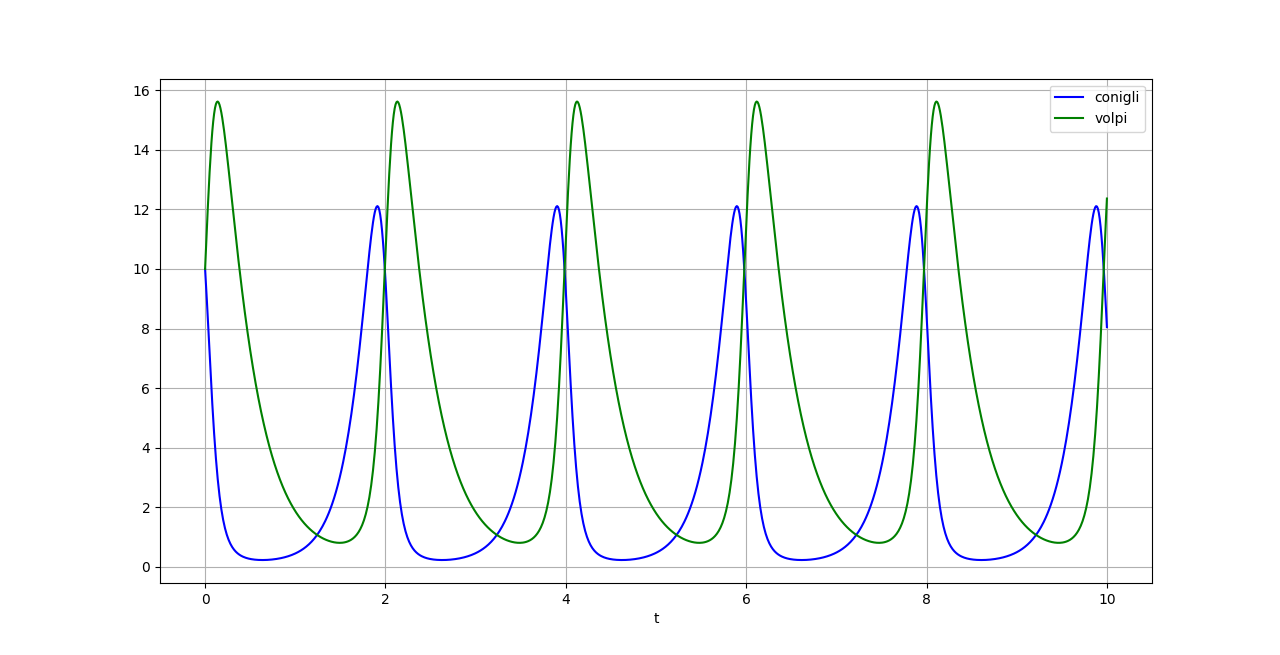
\includegraphics[width=0.4\textwidth]{figures/Volpi-Conigli.png}
\caption{\scriptsize Andamento delle soluzioni (\href{https://github.com/dodogabrie/Sistemi-Complessi/blob/master/python-project/lezione1/volpi_conigli.py}{Link al codice})}
    \label{fig:conigli}
\end{figure}
\noindent
Per una trattazione più rigorosa è necessario notare che le variabili in gioco non sono continue ma bensì discrete (numero di individui di popolazioni).\\
Si passa quindi ad una descrizione probabilistica del sistema che ci porta alla relativa Master Equation.
\begin{center}
    $P(\sigma, t) \in \mathbf{R}$: Probabilità di avere $\sigma \equiv (x,y)\in \mathbf{N}^2$ al tempo $t$.
\end{center}
Inseriamo l'ipotesi di Markov, ovvero che la probabilità che avvenga una transizione tra gli stati del sistema $\sigma \rightarrow \sigma'$ non dipenda dal tempo.
\begin{center}
    $P_r(\sigma\rightarrow\sigma')$: Probabilità di transizione indipendente da $t$.
\end{center}
Dato il sistema al tempo $t$ le probabilità di transizione in un intervallo $\Delta t$ sono:
\[\begin{aligned}
    &P_r(x\to x+1, y) = k_1 c x \Delta t\\
    &P_r(x\to x-1, y \to y+1) = k_2xy\Delta t\\
    &P_r(x\to x,y\to y-1) = k_3 y \Delta t\\
    &P_r(x\to x,y\to y) = 1 - \Delta t \left(k_1cx+ k_2xy + k_3 y\right)
.\end{aligned}\]
Possiamo esprimere la variazione nel tempo della distribuzione di probabilità $P$ tramite le quantità $P_r$:
\begin{redbox}{Esempio di Master Equation}
    Si usa la semplificazione $x^{\pm} \equiv x \pm 1$.
    \begin{equation}
        \begin{aligned}
	    &\frac{P(x,y,t+\Delta  t) - P(x,y,t)}{\Delta  t}  =\\
	    & \quad P_r(x^-\to x, y) \cdot P(x^-,y,t) +\\
	    & \quad P_r(x^+\to x, y^-\to y) \cdot P(x_+,y^-,t) + \\
	    & \quad P_r(x\to x, y^+\to y) P(x,y^+,t) + \\
	    & \quad - \left[1-P_r(x\to x, y\to y)\right]\cdot P(x,y,t) 
        \end{aligned}
    \end{equation}
\end{redbox}
\noindent
Il termine di destra esprime la probabilità di ingresso nello stato $\sigma = (x,y)$ meno la probabilità di uscita da tale stato.
\paragraph{Modello SIR}
Il modello SIR può essere utilizzato per descrivere una situazione pandemica. Gli individui di una popolazione presi in analisi sono:
\begin{itemize}
    \item Suscettibili: $S$.
    \item Infetti: $I$.
    \item Immuni (dopo la malattia): $R$.
\end{itemize}
\[
    \begin{cases}
    S_{n+1} = S_n - \alpha S_n I_n \Delta t\\
    I_{n+1} = I_n + (\alpha S_n I_n - \gamma I_n) \Delta t\\
    R_{n+1} = R_n + \gamma I_n \Delta t
    \end{cases}
\]
Per scrivere la Master Equation si osserva quali sono i termini guidano le transizioni tra i vari stati del sistema:
\[\begin{aligned}
    &P_r(S\to S^-, I \to I^+, R) = \alpha S I \Delta t\\
    &P_r(S, I \to I^-, R \to R^+) = \gamma I \Delta t
.\end{aligned}\]
In modo analogo a quanto fatto per l'esempio precedente si arriva alla seguente equazione:

\begin{align*}
    P(\sigma, &t + \Delta t) = P(\sigma, t) + \\
     + \Delta t &\left[ P(S^+, I^-, R, t) P_r(S^+\to S, I^- \to I, R) + \right.\\
		& \left.+ P(S, I^+, R^-, t) P_r(S, I^+ \to I, R^-\to R) \right] + \\
     - \Delta t & P(\sigma, t) \left[ P_r(S\to S^-, I \to I^+, R) \right. + \\
		& \qquad \qquad \left.+ P_r(S, I\to I^-, R\to R^+)\right].
\end{align*}
A differenza del caso precedente questo sistema ha una configurazione di equilibrio (quando tutti hanno preso il COVID-19 ad esempio).
\paragraph{Rumore shot}%
Ipotizziamo di avere un cavo di rame attraversato da corrente elettrica $J$ e chiamiamo $\sigma$ una sezione di tale cavo ortogonale alla direzione di $J$. Il numero di elettroni che attraversano $\sigma$ sarà soggetto a fluttuazioni, tali fluttuazioni caratterizzano il rumore Shot.\\
La variabile stocastica del problema è $t_k$: il tempo di arrivo di un elettrone su $\sigma$. Ogni elettrone contribuisce alla corrente (misurata su $\sigma$) di una quantità che possiamo schematizzare come una scarica di condensatore $F(t-t_k)$:
\[
    F(t) = \begin{cases}
	0	 			&t<0\\
	q \exp\left(-\alpha t\right) 	&t \ge 0
    \end{cases}
\] 
La corrente totale sarà data dalla somma degli elettroni che arrivano su $\sigma$ per ciascun tempo stocastico $t_k$:
\[
    I(t) = \sum_{t_k}^{} F(t-t_k) 
.\] 
Cerchiamo la Master equation per questo sistema, partiamo dall'ipotesi che in un dato intervallo di tempo $\Delta t$ la probabilità che il numero di elettroni che attraversano $\sigma$ passi da $n$ a $n+1$ sia:
\[
    P(n\to n+1, \text{nell'intervallo }\Delta  t) = \lambda \Delta t
.\] 
Notiamo che gli elettroni scorrono in un'unica direzione, quindi il numero di elettroni che attraversa $\sigma$ può solo aumentare.\\
Il termine della Master Equation $P(n, t + \Delta t)$ si scrive come somma di:
\begin{itemize}
    \item Probabilità di avere già $n$ elettroni al tempo $t$ e che nell'intervallo $\Delta t$ non succeda niente:
	\[
	    (1-\lambda \Delta t) P(n, t)
	\]
    \item La probabilità che al tempo $t$ si hanno $n-1$ elettroni e che nell'intervallo $\Delta t$ ne arrivi un altro:
	\[
	    \lambda \Delta t P(n-1, t)
	\]
\end{itemize}
Quindi mettendo tutto insieme:
\[
    P_n(t+\Delta  t) = \left(1-\lambda\Delta t\right)P_n(t) + \lambda\Delta t  P_{n-1}(t)\implies 
\] 
\[
	\frac{P(n, t+\Delta  t) - P(n,t)}{\Delta t} = \lambda\left[P(n-1,t) -P(n,t)\right] 
.\] 
Che è proprio l'equazione cercata. Vediamo adesso un metodo di risoluzione di questo tipo di equazione.

%%%%%%%%%%%%%%%%%%%%%%%%%%%%%%%%%%%%%%%
%  Metodo della funzione generatrice  %
%%%%%%%%%%%%%%%%%%%%%%%%%%%%%%%%%%%%%%%
\subsection{Metodo della funzione generatrice}%
\label{subsec:fgen_met}
Per risolvere il problema introduciamo la funzione generatrice $G(s,t)$:
\[
    G(s,t) =\sum_{n}^{} s^nP(n,t) 
.\] 
Sostituendo nella master equation del problema precedente nel limite di $\Delta t \to 0$ si ha:
\[
    \frac{\partial G(s,t)}{\partial t} = \lambda (s-1) G(s,t)
.\] 
\[
     \implies  G(s,t) = \exp\left(\lambda (s-1) t\right)G(s,0) 
.\] 
Gli elettroni arrivano per $t\ge 0$, infatti si deve avere che: 
\[
    \begin{cases}
	&P(0,0)=1\\
	&P(n,0) = 0
    \end{cases}
    \ \forall n \implies  G(s,0) = 1 
.\] 
\[\begin{aligned}
    &G(s,t) = e^{\lambda (s-1) t} = \sum_{}^{} s^n P(n,t) \implies  \\
    &\sum e^{-\lambda t} e^{\lambda s t} = \sum_{}^{} e^{-\lambda t}\frac{\left(\lambda ts\right)^n }{n!}  = \sum_{}^{} s^nP(n,t) 
.\end{aligned}\]
In cui si è sfruttato la serie dell'esponenziale $e^{\lambda st}$.
\begin{redbox}{Distribuzione di Poisson}
    \[
	P(n,t)= e^{-\lambda t}\frac{\left(\lambda t\right)^{n}}{n!}
    .\] 
    Dove $P(n,t)$ è la probabilità che al tempo $t$ ci siano $N(t) =n$ elettroni nel sistema.
\end{redbox}
\noindent
Procediamo con il calcolo della corrente, se $N$ è il numero di elettroni arrivati all'istante $t$ allora possiamo definire la quantità:
\[
    \mu(t) \equiv 
    \frac{\text{d} N}{\text{d} t} 
    = \sum_k\delta (t-t_k)  
\] 
Dove $t_k$ è il tempo (random) in cui arriva un elettrone.
Passiamo al continuo nei tempi di arrivo degli elettroni e riscriviamo la corrente come:
\[\begin{aligned}
    I(t) =& \int dx F(t-x) \mu(x) =\\
	 =&\int_{- \infty}^{t} q \exp\left(-\alpha (t-x) \right) \frac{\text{d} N}{\text{d} x} dx 
.\end{aligned}\]
La difficoltà dell'espressione sta nel fatto che $N(t)$ è una funzione a gradini con i gradini che arrivano in modo stocastico nel tempo.\\
Si deriva a destra e sinistra rispetto al tempo ed si integra per parti:
\[\begin{aligned}
    \frac{\text{d} I}{\text{d} t} &= \left[q\exp\left(-\alpha (t-x)\right)\left. \frac{\text{d} N}{\text{d} t}\right]  \right|_{x=t} + \\
				   &\qquad +\int_{-\infty}^{t} \left(-\alpha q\right)\exp\left(-\alpha (t-x)\right)\frac{\text{d} N}{\text{d} x} dx =\\
				   &= q\mu (t) - \alpha I(t) 
.\end{aligned}\]
\begin{redbox}{Equazione stocastica differenziale}
 \[
    \frac{\text{d} I}{\text{d} t} = -\alpha I(t) + q\mu (t) 
.\]    
\end{redbox}
\noindent
Il termine in $\mu$ dipende dalla sequenza casuale di $\delta(t-t_k)$, ognuna di queste può dare soluzioni differenti.\\ 
Rispetto al moto Browniano visto in precedenza, in cui si aveva che $f(\Delta) = f(-\Delta)$, adesso abbiamo un processo che evolve solo in avanti.\\
L'idea per risolvere il problema è di interpolare l'andamento di $N$ con un moto browniano, prendendo la media e le fluttuazioni del termine stocastico.
Essendo il termine in $\mu$ la derivata di un processo poissoniano abbiamo le seguenti proprietà:
\[\begin{aligned}
    &\left<\mu dt\right>=\left<dN\right> = \lambda dt\\
    & \left<\left(\lambda dt - \mu dt\right)^2\right> = \lambda dt
.\end{aligned}\]
Si cerca di scrivere questo processo stocastico (unilaterale) come un processo di Langevin, quindi si definisce una nuova variabile stocastica $d\eta = dN - \lambda dt$.
\[
    dN = \lambda dt + d\eta	
.\] 
Questo equivale a scomporre il processo a salti $dN$ in un drift lineare ($\lambda dt$) ed una fluttuazione stocastica ($d\eta$).\\
Il differenziale della corrente si scrive come:
\[
    dI(t) = \left(\lambda q-\alpha I\right)dt+ qd\eta (t) 
.\] 
In questo modo la variabile stocastica $d\eta$ gode delle seguenti proprietà:
\begin{itemize}
    \item $\left<d\eta \right> = 0$
    \item $\left<d\eta^2 \right> = \lambda dt$
    \item $\left<I d\eta \right> = 0$
\end{itemize}
\[
    \frac{\text{d} }{\text{d} t} \left<I\right> = \lambda q -\alpha\left<I\right>
.\] 
Il risultato stazionario per l'equazione è:
\[
    \left<I\right>_{\infty}=\frac{\lambda q}{\alpha}
.\] 
Procediamo con una ipotesi sbagliata: trascurare le fluttuazioni nel seguente termine
\begin{equation}
    \left(I+dI\right)^2 \approx I^2 + 2IdI	\label{eq:baddiff}
\end{equation}
Quindi con il risultato che dovrebbe esser noto sui differenziali: $d\left(I^2\right) = 2IdI$, se assumiamo questo e moltiplichiamo a destra e sinistra per $\left<I\right>$ nella equazione   per la corrente otteniamo:
\[
    \frac{1}{2}\frac{\text{d} }{\text{d} t} \left<I^2\right>= \lambda q\left<I\right>-\alpha\left<I^2\right>
.\] 
Che ci porta a concludere che:
\[
    \left<I^2\right>_{\infty} = \frac{\lambda q}{\alpha}\left<I\right>_{\infty} = \left(\left<I\right>_{\infty}\right)^2
.\] 
Otteniamo quindi un paradosso, la corrente ha varianza nulla:
\[
  \left<I^2\right>-\left<I\right>^2 = 0  
.\] 
Questo significherebbe che la "larghezza" del moto Browniano è nulla, quindi la corrente sarebbe costante e continua.\\
L'errore è dovuto al differenziale \ref{eq:baddiff}, infatti il termine trascurato vale:
\[
    \left<dI^2\right> = \left<q^2d\eta^2\right> = q^2\lambda dt
.\] 
Che è anch'esso di prim'ordine nel tempo! L'equazione corretta sarebbe allora:
\[
    \frac{1}{2}\frac{\text{d} }{\text{d} t} \left<I^2\right>= \lambda q\left<I\right>-\alpha\left<I^2\right> + q^2\lambda + O(dt)
.\]
\newpage
